%%%%%%%%%%%%%%%%%%%%%%%%%%%%%%%%%%%%

\section{ロジスティック回帰}

%%%%%%%%%%%%%%%%%%%%%%%%%%%%%%%%%%%%

\begin{frame}
\frametitle{これまでの回帰 ...}

ここまでに扱った内容：

{\small
\begin{itemize}
\item 単純線形回帰
\begin{itemize}
\item 数値応答変数と数値またはカテゴリ予測変数の関係
\end{itemize}
\item 重回帰
\begin{itemize}
\item 数値応答変数と複数の数値およびカテゴリ予測変数の関係
\end{itemize}
\end{itemize}
}

まだ扱っていないのは、予測変数が変わった形（非線形、複雑な依存構造など）であったり、応答変数が変わった形（カテゴリ変数、カウントデータなど）であったりする場合の対処法である。


\end{frame}

%%%%%%%%%%%%%%%%%%%%%%%%%%%%%%%%%%%

\begin{frame}
\frametitle{オッズ}

\vspace{-2mm}

オッズは事象の確率を表す別の方法であり、ギャンブル（およびロジスティック回帰）でよく使われる。\\

~\\

\formula{オッズ}
{
ある事象 $E$ に対して、
{\small
\[\text{odds}(E) = \frac{P(E)}{P(E^c)} = \frac{P(E)}{1-P(E)}\]
}
同様に、E のオッズが $x$ 対 $y$ であると言われたなら
{\small
\[\text{odds}(E) = \frac{x}{y} = \frac{x/(x+y)}{y/(x+y)} \]
}
これは次のことを意味する
{\small
\[P(E) = x/(x+y),\quad P(E^c) = y/(x+y)\]
}
}

\end{frame}

%%%%%%%%%%%%%%%%%%%%%%%%%%%%%%%%%%%

\subsection{一般化線形モデル}

%%%%%%%%%%%%%%%%%%%%%%%%%%%%%%%%%%%

\begin{frame}
\frametitle{例 --- ドナー隊}

1846年、ドナー家とリード家はイリノイ州スプリングフィールドをカバーワゴンでカリフォルニアに向けて出発した。7月、後に「ドナー隊」として知られることになるこの一行はワイオミング州フォートブリジャーに到達した。そこでリーダーたちはサクラメントバレーへの新しい未開拓ルートを試みることを決定した。87人と20台のワゴンという最大規模に達した一行は、ワサッチ山脈の困難な横断と、グレートソルト湖西側の砂漠横断で再び遅延した。10月下旬に激しい降雪がこの地域を襲い、グループはシエラネバダ山脈東部に立ち往生した。最後の生存者が1847年4月21日に救助されるまでに、87人のうち40人が飢餓と極寒により死亡した。\\


\vfill

{\tiny From \textit{Ramsey, F.L. and Schafer, D.W. (2002). The Statistical Sleuth: A Course in Methods of Data Analysis (2nd ed)}}
\end{frame}


%%%%%%%%%%%%%%%%%%%%%%%%%%%%%%%%%%%

\begin{frame}
\frametitle{例 --- ドナー隊 --- データ}

\begin{center}
\begin{tabular}{rlll}
  \hline
     & Age   & Sex    & Status \\
  \hline
   1 & 23.00 & Male   & Died \\
   2 & 40.00 & Female & Survived \\
   3 & 40.00 & Male   & Survived \\
   4 & 30.00 & Male   & Died \\
   5 & 28.00 & Male   & Died \\
\vdots & ~~~\vdots & ~~~\vdots & ~~~\vdots \\
  43 & 23.00 & Male   & Survived \\
  44 & 24.00 & Male   & Died \\
  45 & 25.00 & Female & Survived \\
   \hline
\end{tabular}
\end{center}

\end{frame}

%%%%%%%%%%%%%%%%%%%%%%%%%%%%%%%%%%%
\begin{frame}
\frametitle{例 --- ドナー隊 --- 探索的データ分析}

生存状況 vs. 性別：\\

\begin{center}
\begin{tabular}{rrr}
\hline
         & Male & Female \\
\hline
Died     &  20  &   5 \\
Survived &  10  &  10 \\
   \hline
\end{tabular}
\end{center}

\vfill

生存状況 vs. 年齢：\\
\begin{center}
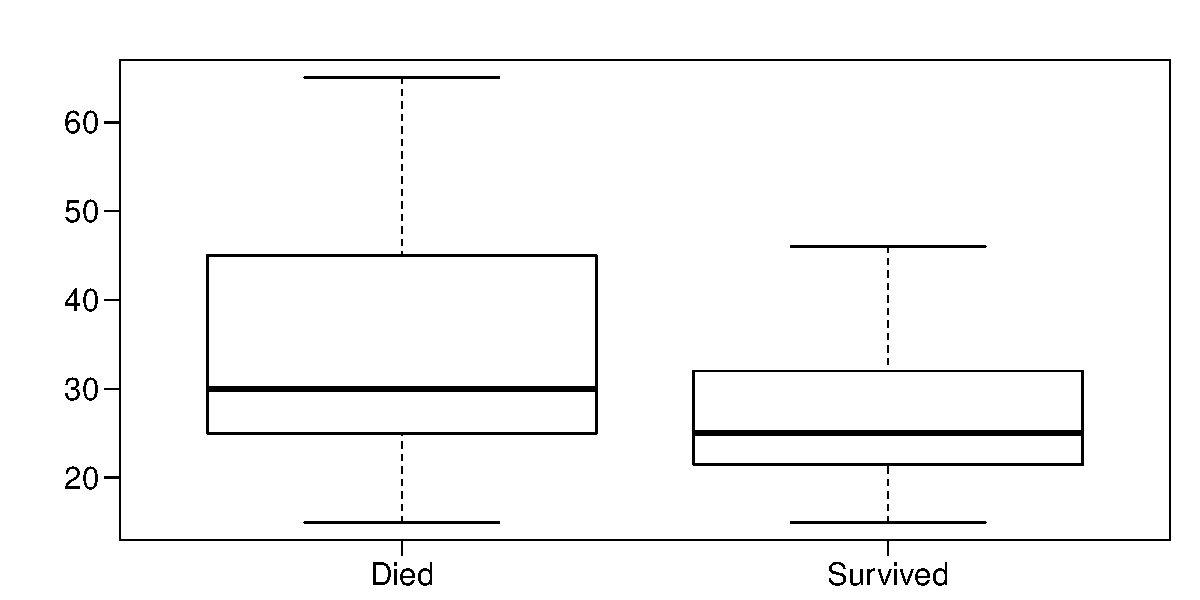
\includegraphics[width=0.8\textwidth]{9-5_logistic_reg/figures/donner/status_age}
\end{center}

\end{frame}

%%%%%%%%%%%%%%%%%%%%%%%%%%%%%%%%%%%

\begin{frame}
\frametitle{例 --- ドナー隊}

年齢と性別の両方が生存に影響を与えることは明らかだが、この関係を探るためのモデルをどのように作ればよいか？\\

~\\

死亡を 0、生存を 1 に設定しても、変換で解決できる問題ではない --- より高度な手法が必要である。

~\\

問題の捉え方の1つとして --- 生存と死亡を、確率が線形モデルの変換で与えられる二項分布から生じる成功と失敗として扱うことができる。

\end{frame}

%%%%%%%%%%%%%%%%%%%%%%%%%%%%%%%%%%%

\begin{frame}
\frametitle{一般化線形モデル}

これは回帰におけるこの種の問題に対処する非常に一般的な方法であり、結果として得られるモデルを一般化線形モデル（GLM）と呼ぶ。ロジスティック回帰はこのタイプのモデルの一例に過ぎない。\\
~\\
すべての一般化線形モデルは以下の3つの特性を持つ：
\begin{enumerate}
\item 応答変数を記述する確率分布
\item 線形モデル
\begin{itemize}
\item $\eta = \beta_0+\beta_1 X_1 + \cdots + \beta_n X_n$
\end{itemize}
\item 線形モデルと応答分布のパラメータを結びつけるリンク関数
\begin{itemize}
\item $g(p) = \eta$ または $p = g^{-1}(\eta)$
\end{itemize}
\end{enumerate}

\end{frame}

%%%%%%%%%%%%%%%%%%%%%%%%%%%%%%%%%%%

\subsection{ロジスティック回帰}

%%%%%%%%%%%%%%%%%%%%%%%%%%%%%%%%%%%

\begin{frame}
\frametitle{ロジスティック回帰}

ロジスティック回帰は、数値変数とカテゴリ変数の予測変数を用いて2値のカテゴリ応答変数をモデル化するための GLM である。\\
~\\
応答変数が二項分布から生じると仮定し、所与の予測変数セットに対する成功確率 $p$ をモデル化したい。\\
~\\

ロジスティックモデルの定式化を完成させるために、$\eta$ と $p$ を結びつける適切なリンク関数を設定する必要がある。様々な選択肢があるが、最もよく使われるのはロジット関数である。\\

~\\

\formula{ロジット関数}{
\[logit(p) = \log\left(\frac{p}{1-p}\right),\text{ ただし $0\le p \le 1$}\]
}

\end{frame}

%%%%%%%%%%%%%%%%%%%%%%%%%%%%%%%%%%%

\begin{frame}
\frametitle{ロジットの性質}

ロジット関数は 0 から 1 の間の値を取り、$-\infty$ から $\infty$ の値にマッピングする。\\
~\\

\formula{逆ロジット（ロジスティック）関数}
{
\[g^{-1}(x) = \frac{\exp(x)}{1+\exp(x)} = \frac{1}{1+\exp(-x)}\]
}

~\\
逆ロジット関数は $-\infty$ から $\infty$ の間の値を取り、0 から 1 の値にマッピングする。\\

~\\
この定式化はモデルの解釈にも有用で、ロジットは成功の対数オッズとして解釈できる（詳細は後述）。


\end{frame}

%%%%%%%%%%%%%%%%%%%%%%%%%%%%%%%%%%%

\begin{frame}
\frametitle{ロジスティック回帰モデル}

GLM の3つの基準から得られる：

\begin{align*}
y_i &\sim \text{Binom}(p_i)\\
\\
\eta &= \beta_0+\beta_1 x_1 + \cdots + \beta_n x_n\\
\\
\text{logit}(p) &= \eta
\end{align*}

ここから次の式が導かれる：

\[ p_i = \frac{\exp(\beta_0+\beta_1 x_{1,i} + \cdots + \beta_n x_{n,i})}{1+\exp(\beta_0+\beta_1 x_{1,i} + \cdots + \beta_n x_{n,i})} \]


\end{frame}

%%%%%%%%%%%%%%%%%%%%%%%%%%%%%%%%%%%

\begin{frame}[fragile]
\frametitle{例 --- ドナー隊 --- モデル}
\vspace{-2mm}
R では、\var{lm} の代わりに \var{glm} を使い、\var{family} 引数で適合する GLM の種類を指定することで、線形モデルと同様の方法で GLM を適合できる。\\

\vspace{2mm}

{\scriptsize
\begin{verbatim}
summary(glm(Status ~ Age, data=donner, family=binomial))

## Call:
## glm(formula = Status ~ Age, family = binomial, data = donner)
##
## Coefficients:
##             Estimate Std. Error z value Pr(>|z|)
## (Intercept)  1.81852    0.99937   1.820   0.0688 .
## Age         -0.06647    0.03222  -2.063   0.0391 *
##
##     Null deviance: 61.827  on 44  degrees of freedom
## Residual deviance: 56.291  on 43  degrees of freedom
## AIC: 60.291
##
## Number of Fisher Scoring iterations: 4
\end{verbatim}
}
\end{frame}


%%%%%%%%%%%%%%%%%%%%%%%%%%%%%%%%%%%

\begin{frame}
\frametitle{例 --- ドナー隊 --- 予測}

{\scriptsize
\begin{center}
\begin{tabular}{rrrrr}
  \hline
 & Estimate & Std. Error & z value & Pr($>$$|$z$|$) \\
  \hline
(Intercept) & 1.8185 & 0.9994 & 1.82 & 0.0688 \\
  Age & -0.0665 & 0.0322 & -2.06 & 0.0391 \\
   \hline
\end{tabular}
\end{center}
}

モデル：
\[\log\left(\frac{p}{1-p}\right) = 1.8185-0.0665\times \text{Age}\]

~\\~\\
新生児（Age=0）の生存オッズ/確率：
{\scriptsize
\begin{align*}
\log\left(\frac{p}{1-p}\right) &= 1.8185-0.0665\times \orange{0}\\
\frac{p}{1-p} &= \exp(1.8185) = 6.16 \\
p &= 6.16/7.16 = 0.86
\end{align*}
}

\end{frame}

%%%%%%%%%%%%%%%%%%%%%%%%%%%%%%%%%%%

\begin{frame}
\frametitle{例 --- ドナー隊 --- 予測（続き）}

モデル：
{\scriptsize
\[\log\left(\frac{p}{1-p}\right) = 1.8185-0.0665\times \text{Age}\]
}

25歳の生存オッズ/確率：
{\scriptsize
\begin{align*}
\log\left(\frac{p}{1-p}\right) &= 1.8185-0.0665\times \orange{25}\\
\frac{p}{1-p} &= \exp(0.156) = 1.17 \\
p &= 1.17/2.17 = 0.539
\end{align*}
}

50歳の生存オッズ/確率：
{\scriptsize
\begin{align*}
\log\left(\frac{p}{1-p}\right) &= 1.8185-0.0665\times \orange{50}\\
\frac{p}{1-p} &= \exp(-1.5065) = 0.222 \\
p &= 0.222/1.222 =  0.181
\end{align*}
}

\end{frame}

%%%%%%%%%%%%%%%%%%%%%%%%%%%%%%%%%%%

\begin{frame}
\frametitle{例 --- ドナー隊 --- 予測（続き）}

{\scriptsize
\[\log\left(\frac{p}{1-p}\right) = 1.8185-0.0665\times \text{Age}\]
}

\vspace{-10mm}

\begin{center}
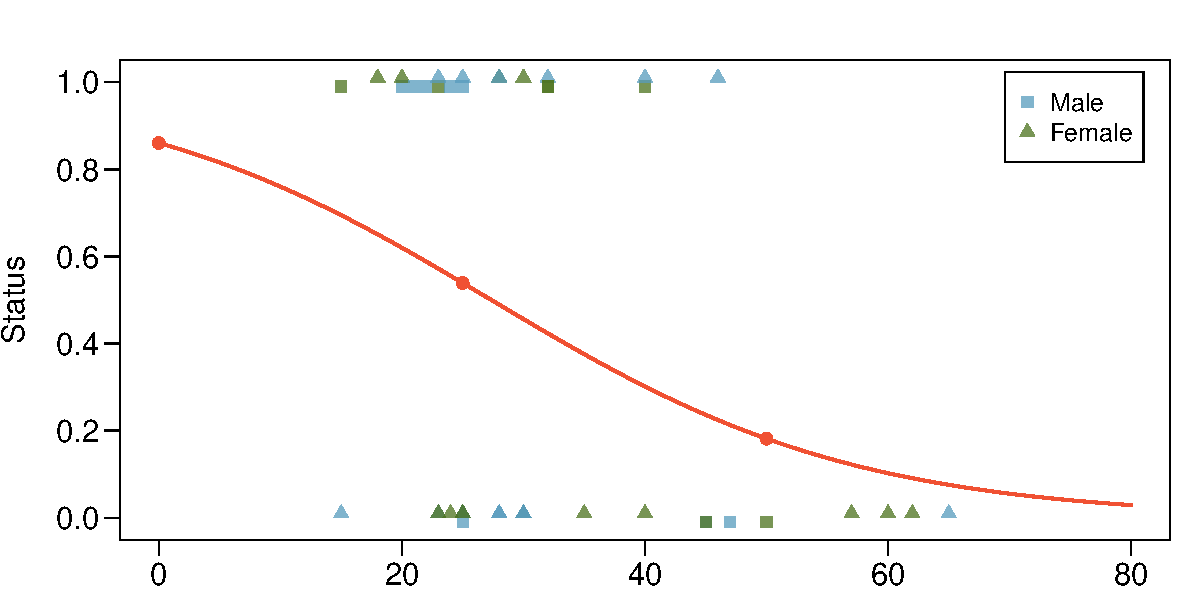
\includegraphics[width=0.8\textwidth]{9-5_logistic_reg/figures/donner/donner_scatter_pred.pdf}
\end{center}
\end{frame}

%%%%%%%%%%%%%%%%%%%%%%%%%%%%%%%%%%%

\begin{frame}
\frametitle{例 --- ドナー隊 --- 解釈}

{\scriptsize
\begin{center}
\begin{tabular}{rrrrr}
  \hline
 & Estimate & Std. Error & z value & Pr($>$$|$z$|$) \\
  \hline
(Intercept) & 1.8185 & 0.9994 & 1.82 & 0.0688 \\
  Age & -0.0665 & 0.0322 & -2.06 & 0.0391 \\
   \hline
\end{tabular}
\end{center}
}

単純な解釈は切片と傾きの項について、対数オッズと対数オッズ比の観点でのみ可能である。\\

~\\

\hl{切片}：年齢 0 のメンバーの生存の対数オッズ。ここからオッズや確率を計算できるが、追加計算が必要である。\\

~\\

\hl{傾き}：年齢が 1 単位増加する（1歳年上になる）と対数オッズ比がどれだけ変化するか。直感的には分かりにくい。多くの場合、符号と相対的な大きさのみを気にする。

\end{frame}

%%%%%%%%%%%%%%%%%%%%%%%%%%%%%%%%%%%

\begin{frame}[fragile]
\frametitle{例 --- ドナー隊 --- 解釈 --- 傾き}

{\scriptsize
\begin{align*}
\log\left(\frac{p_1}{1-p_1}\right) &= 1.8185-0.0665 (x+1) \\
                                   &= 1.8185-0.0665 x-0.0665 \\
\log\left(\frac{p_2}{1-p_2}\right) &= 1.8185-0.0665 x \\
\\
\log\left(\frac{p_1}{1-p_1}\right) - \log\left(\frac{p_2}{1-p_2}\right) &= -0.0665 \\
\log\left(\left. \frac{p_1}{1-p_1} \right/ \frac{p_2}{1-p_2} \right) &= -0.0665 \\
\left. \frac{p_1}{1-p_1} \right/ \frac{p_2}{1-p_2} &= \exp(-0.0665) = 0.94
\end{align*}
}

\end{frame}

%%%%%%%%%%%%%%%%%%%%%%%%%%%%%%%%%%%

\begin{frame}[fragile]
\frametitle{例 --- ドナー隊 --- 年齢と性別}
\vspace{-3mm}
{\tiny
\begin{verbatim}
summary(glm(Status ~ Age + Sex, data=donner, family=binomial))

## Call:
## glm(formula = Status ~ Age + Sex, family = binomial, data = donner)
##
## Coefficients:
##             Estimate Std. Error z value Pr(>|z|)
## (Intercept)  1.63312    1.11018   1.471   0.1413
## Age         -0.07820    0.03728  -2.097   0.0359 *
## SexFemale    1.59729    0.75547   2.114   0.0345 *
## ---
##
## (Dispersion parameter for binomial family taken to be 1)
##
##     Null deviance: 61.827  on 44  degrees of freedom
## Residual deviance: 51.256  on 42  degrees of freedom
## AIC: 57.256
##
## Number of Fisher Scoring iterations: 4
\end{verbatim}
}

\hl{性別の傾き}：他の予測変数を一定に保つとき、これは与えられた水準（Female）と参照水準（Male）の対数オッズ比である。

\end{frame}

%%%%%%%%%%%%%%%%%%%%%%%%%%%%%%%%%%%

\begin{frame}
\frametitle{例 --- ドナー隊 --- 性別別モデル}

重回帰と同様に、性別を代入することで男女それぞれの生存状況 vs. 年齢のモデルを得ることができる。\\
~\\

一般モデル：
{\scriptsize
\[\log\left(\frac{p_1}{1-p_1}\right) = 1.63312 + -0.07820\times\text{Age} + 1.59729\times\text{Sex}\]
}

男性モデル：
{\scriptsize
\begin{align*}
\log\left(\frac{p_1}{1-p_1}\right) &= 1.63312 + -0.07820\times\text{Age} + 1.59729\times\orange{0}\\
                                   &= 1.63312 + -0.07820\times\text{Age}
\end{align*}
}

女性モデル：
{\scriptsize
\begin{align*}
\log\left(\frac{p_1}{1-p_1}\right) &= 1.63312 + -0.07820\times\text{Age} + 1.59729\times\orange{1}\\
                                   &= 3.23041 + -0.07820\times\text{Age}
\end{align*}
}

\end{frame}

%%%%%%%%%%%%%%%%%%%%%%%%%%%%%%%%%%%

\begin{frame}
\frametitle{例 --- ドナー隊 --- 性別別モデル（続き）}

\begin{center}
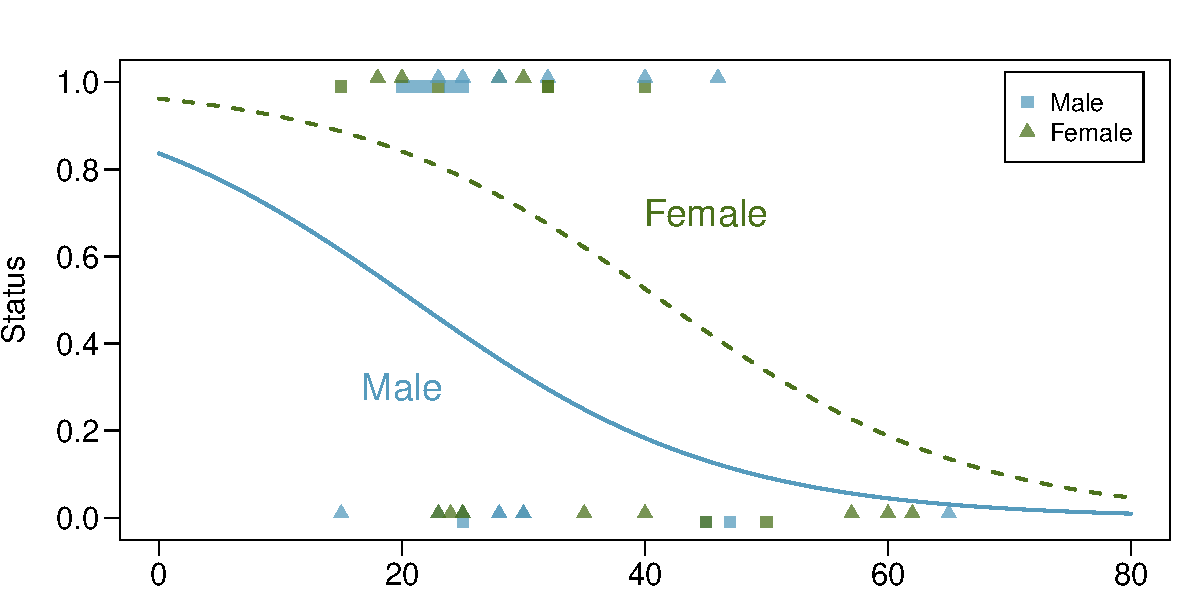
\includegraphics[width=\textwidth]{9-5_logistic_reg/figures/donner/donner_scatter_both.pdf}
\end{center}

\end{frame}

%%%%%%%%%%%%%%%%%%%%%%%%%%%%%%%%%%%

%%%%%%%%%%%%%%%%%%%%%%%%%%%%%%%%%%%

\begin{frame}[fragile,shrink]
\frametitle{モデル全体の仮説検定}
\vspace{-3mm}
{\scriptsize
\begin{verbatim}
summary(glm(Status ~ Age + Sex, data=donner, family=binomial))

## Call:
## glm(formula = Status ~ Age + Sex, family = binomial, data = donner)
##
## Coefficients:
##             Estimate Std. Error z value Pr(>|z|)
## (Intercept)  1.63312    1.11018   1.471   0.1413
## Age         -0.07820    0.03728  -2.097   0.0359 *
## SexFemale    1.59729    0.75547   2.114   0.0345 *
## ---
##
## (Dispersion parameter for binomial family taken to be 1)
##
##     Null deviance: 61.827  on 44  degrees of freedom
## Residual deviance: 51.256  on 42  degrees of freedom
## AIC: 57.256
##
## Number of Fisher Scoring iterations: 4
\end{verbatim}
}

\Note{モデル出力には F 統計量が含まれていない。一般的なルールとして、GLM モデルにはモデル全体の仮説検定が存在しない。}

\end{frame}

%%%%%%%%%%%%%%%%%%%%%%%%%%%%%%%%%%%

\begin{frame}
\frametitle{係数の仮説検定}

\begin{center}
\begin{tabular}{rrrrr}
  \hline
 & Estimate & Std. Error & z value & Pr($>$$|$z$|$) \\
  \hline
(Intercept) & 1.6331 & 1.1102 & 1.47 & 0.1413 \\
  Age & -0.0782 & 0.0373 & -2.10 & 0.0359 \\
  SexFemale & 1.5973 & 0.7555 & 2.11 & 0.0345 \\
   \hline
\end{tabular}
\end{center}

ただし、個々の係数についての推測は依然として可能であり、基本的な設定はこれまでに見てきたものとまったく同じだが、Z 検定を使用する。\\

~\\

\Note{唯一の難点は、このコースの範囲をはるかに超えるが、標準誤差の計算方法である。}

\end{frame}

%%%%%%%%%%%%%%%%%%%%%%%%%%%%%%%%%%%

\begin{frame}
\frametitle{年齢の傾き係数の検定}

{\small
\begin{center}
\begin{tabular}{rrrrr}
  \hline
            & Estimate & Std. Error & z value & Pr($>$$|$z$|$) \\
  \hline
(Intercept) & 1.6331  & 1.1102 & 1.47 & 0.1413 \\
        Age & \orange{-0.0782} & \green{0.0373} & \orange{-2.10} & \textcolor{blue}{0.0359} \\
  SexFemale & 1.5973  & 0.7555 & 2.11 & 0.0345 \\
   \hline
\end{tabular}
\end{center}
}

\begin{align*}
H_0:~& \beta_{age} = 0 \\
H_A:~& \beta_{age} \ne 0
\end{align*}

\begin{align*}
Z &= \frac{\hat{\beta_{age}} - \beta_{age}}{SE_{age}}
   = \frac{\orange{-0.0782} - 0}{\green{0.0373}} = \orange{-2.10} \\
\\
\text{p-value} &= P(|Z| > \orange{2.10}) = P(Z>\orange{2.10})+P(Z<\orange{-2.10})\\
               &= 2\times 0.0178 = \textcolor{blue}{0.0359}
\end{align*}

\end{frame}

%%%%%%%%%%%%%%%%%%%%%%%%%%%%%%%%%%%

%%%%%%%%%%%%%%%%%%%%%%%%%%%%%%%%%%%

\begin{frame}
\frametitle{年齢の傾き係数の信頼区間}

\begin{center}
\begin{tabular}{rrrrr}
  \hline
 & Estimate & Std. Error & z value & Pr($>$$|$z$|$) \\
  \hline
(Intercept) & 1.6331 & 1.1102 & 1.47 & 0.1413 \\
  Age & -0.0782 & 0.0373 & -2.10 & 0.0359 \\
  SexFemale & 1.5973 & 0.7555 & 2.11 & 0.0345 \\
   \hline
\end{tabular}
\end{center}

傾きの解釈は、予測変数の 1 単位の変化に対する対数オッズ比の変化であることを覚えておく。\\
~\\

対数オッズ比：
\[ CI = PE \pm CV \times SE = -0.0782 \pm 1.96 \times 0.0373 = (-0.1513,  -0.0051) \]

オッズ比：
\[ \exp(CI) = (\exp{-0.1513}, \exp{-0.0051}) = (0.8596,\ 0.9949) \]


\end{frame}


%%%%%%%%%%%%%%%%%%%%%%%%%%%%%%%%%%%

\subsection{追加例}

%%%%%%%%%%%%%%%%%%%%%%%%%%%%%%%%%%%


\begin{frame}
\frametitle{例 --- 野鳥飼育と肺がん}

1972〜1981年にオランダのハーグで実施された健康調査により、ペットの鳥の飼育と肺がんリスクの増加との関連が発見された。鳥の飼育をリスク因子として調査するために、研究者らは1985年にハーグ（人口45万人）の4つの病院で症例対照研究を実施した。彼らは一般開業医に登録されており、65歳以下で、1965年以降ハーグに居住していた患者の中から49例の肺がん症例を特定した。また、同じ年齢構成を持つ住民から98人の対照を選んだ。


\vfill

{\tiny From \textit{Ramsey, F.L. and Schafer, D.W. (2002). The Statistical Sleuth: A Course in Methods of Data Analysis (2nd ed)}}
\end{frame}

%%%%%%%%%%%%%%%%%%%%%%%%%%%%%%%%%%%

\begin{frame}
\frametitle{例 --- 野鳥飼育と肺がん --- データ}

{\scriptsize
\begin{tabular}{rllllrrr}
  \hline
    & \var{LC} & \var{FM} & \var{SS} & \var{BK} & \var{AG} & \var{YR} & \var{CD} \\
  \hline
  1 & LungCancer & Male & Low & Bird & 37.00 & 19.00 & 12.00 \\
  2 & LungCancer & Male & Low & Bird & 41.00 & 22.00 & 15.00 \\
  3 & LungCancer & Male & High & NoBird & 43.00 & 19.00 & 15.00 \\
\vdots & ~~~~~~\vdots & ~~~\vdots & ~~\vdots & ~~~\vdots & \vdots~~~ & \vdots~~~ & \vdots~~~ \\
147 & NoCancer & Female & Low & NoBird & 65.00 & 7.00 & 2.00 \\
   \hline
\end{tabular}
}

{\small
\begin{center}
\begin{tabular}{ll}
\var{LC} & 肺がんの有無 \\
\var{FM} & 対象者の性別 \\
\var{SS} & 社会経済的状況 \\
\var{BK} & 鳥の飼育の有無 \\
\var{AG} & 対象者の年齢（歳） \\
\var{YR} & 診断または検査前の喫煙年数 \\
\var{CD} & 平均喫煙率（1日当たりの本数）
\end{tabular}
\end{center}
}

\Note{NoCancer が参照応答（0 または失敗）、LungCancer が非参照応答（1 または成功）--- これは解釈に重要である。}

\end{frame}

%%%%%%%%%%%%%%%%%%%%%%%%%%%%%%%%%%%

\begin{frame}
\frametitle{例 --- 野鳥飼育と肺がん --- 探索的データ分析}

\begin{center}
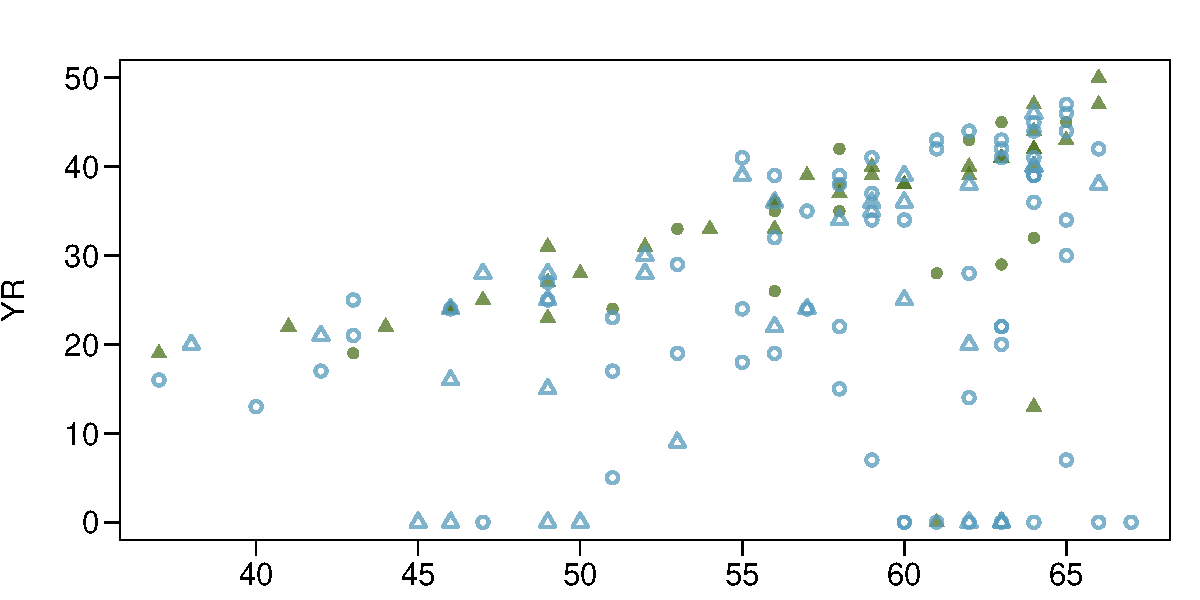
\includegraphics[width=0.8\textwidth]{9-5_logistic_reg/figures/birds/birds.pdf}
\end{center}

{\scriptsize
\begin{center}
\begin{tabular}{r|cc}
               & Bird（鳥あり）& No Bird（鳥なし）\\
\hline
Lung Cancer（肺がん）    & \textcolor{oiG}{$\blacktriangle$} & \textcolor{oiG}{$\bullet$} \\
No Lung Cancer（肺がんなし）& \textcolor{oiB}{$\triangle$}      & \textcolor{oiB}{$\circ$}
\end{tabular}
\end{center}
}



\end{frame}

%%%%%%%%%%%%%%%%%%%%%%%%%%%%%%%%%%%

\begin{frame}[fragile]
\frametitle{例 --- 野鳥飼育と肺がん --- モデル}

\vspace{-5mm}

{\tiny
\begin{verbatim}
summary(glm(LC ~ FM + SS + BK + AG + YR + CD, data=bird, family=binomial))

## Call:
## glm(formula = LC ~ FM + SS + BK + AG + YR + CD, family = binomial,
##     data = bird)
##
## Coefficients:
##             Estimate Std. Error z value Pr(>|z|)
## (Intercept) -1.93736    1.80425  -1.074 0.282924
## FMFemale     0.56127    0.53116   1.057 0.290653
## SSHigh       0.10545    0.46885   0.225 0.822050
## BKBird       1.36259    0.41128   3.313 0.000923 ***
## AG          -0.03976    0.03548  -1.120 0.262503
## YR           0.07287    0.02649   2.751 0.005940 **
## CD           0.02602    0.02552   1.019 0.308055
##
## (Dispersion parameter for binomial family taken to be 1)
##
##     Null deviance: 187.14  on 146  degrees of freedom
## Residual deviance: 154.20  on 140  degrees of freedom
## AIC: 168.2
##
## Number of Fisher Scoring iterations: 5
\end{verbatim}
}

\end{frame}

%%%%%%%%%%%%%%%%%%%%%%%%%%%%%%%%%%%

\begin{frame}
\frametitle{例 --- 野鳥飼育と肺がん --- 解釈}

\vspace{-5mm}

{\scriptsize
\begin{center}
\begin{tabular}{rrrrr}
  \hline
 & Estimate & Std. Error & z value & Pr($>$$|$z$|$) \\
  \hline
(Intercept) & -1.9374 & 1.8043 & -1.07 & 0.2829 \\
  FMFemale  & 0.5613 & 0.5312 & 1.06 & 0.2907 \\
  SSHigh    & 0.1054 & 0.4688 & 0.22 & 0.8221 \\
\rowcolor{gray}
  BKBird    & 1.3626 & 0.4113 & 3.31 & 0.0009 \\
  AG        & -0.0398 & 0.0355 & -1.12 & 0.2625 \\
\rowcolor{gray}
  YR        & 0.0729 & 0.0265 & 2.75 & 0.0059 \\
  CD        & 0.0260 & 0.0255 & 1.02 & 0.3081 \\
   \hline
\end{tabular}
\end{center}
}

他のすべての予測変数を一定に保つと、
\begin{itemize}
\item 鳥を飼育している人と飼育していない人の肺がんに関するオッズ比は $\exp(1.3626) = 3.91$ である。
\item 喫煙年数が 1 年増加することによる肺がんのオッズ比は $\exp(0.0729) = 1.08$ である。
\end{itemize}

\end{frame}

%%%%%%%%%%%%%%%%%%%%%%%%%%%%%%%%%%%

\begin{frame}
\frametitle{数値が意味しないこと ...}

ロジスティック回帰の解釈でよくある間違いは、オッズ比を確率の比として扱うことである。\\

~\\

鳥を飼育している人は、飼育していない人より肺がんを発症する可能性が 4 倍高いわけでは\emph{ない}。

~\\

これはリスク比とオッズ比の違いである。


\[RR = \frac{P(\text{疾患} | \text{曝露あり})}{P(\text{疾患} | \text{曝露なし})} \]

\[OR = \frac{P(\text{疾患} | \text{曝露あり}) / [1-P(\text{疾患} | \text{曝露あり})]}{P(\text{疾患} | \text{曝露なし})/[1-P(\text{疾患} | \text{曝露なし})]} \]


\end{frame}

%%%%%%%%%%%%%%%%%%%%%%%%%%%%%%%%%%%

\begin{frame}
\frametitle{鳥の話に戻る}

$P(\text{肺がん}|\text{鳥なし}) = 0.05$ とわかっている場合、鳥を飼育している人の肺がん確率は？

\begin{align*}
OR &= \frac{P(\text{肺がん} | \text{鳥あり}) / [1-P(\text{肺がん} | \text{鳥あり})]}{P(\text{肺がん} | \text{鳥なし})/[1-P(\text{肺がん} | \text{鳥なし})]} \\
\\
   &= \frac{P(\text{肺がん} | \text{鳥あり}) / [1-P(\text{肺がん} | \text{鳥あり})]}{0.05/[1-0.05]} = 3.91
\end{align*}

\[ P(\text{肺がん} | \text{鳥あり}) =  \frac{3.91 \times \frac{0.05}{0.95}}{1+3.91 \times \frac{0.05}{0.95}} = 0.171\]

\[ RR = P(\text{肺がん} | \text{鳥あり}) / P(\text{肺がん} | \text{鳥なし}) = 0.171 / 0.05 = 3.41\]

\end{frame}

%%%%%%%%%%%%%%%%%%%%%%%%%%%%%%%%%%

\begin{frame}
\frametitle{鳥の OR 曲線}

\vspace{-8mm}

\begin{center}
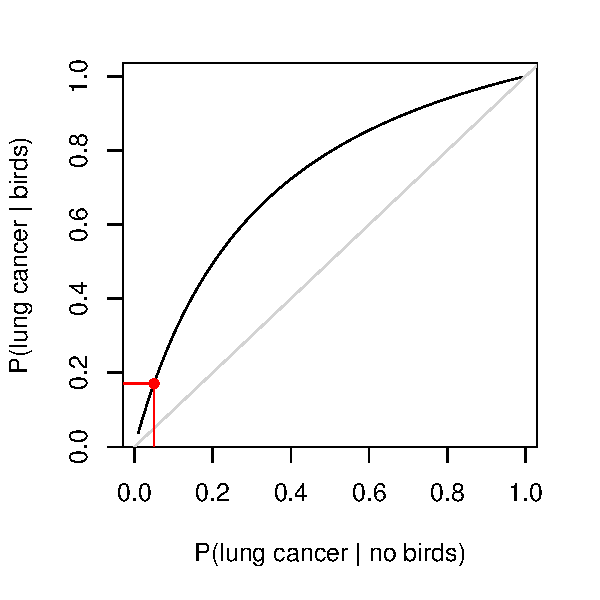
\includegraphics[width=0.7\textwidth]{9-5_logistic_reg/figures/birds/OR3.pdf}
\end{center}

\end{frame}

%%%%%%%%%%%%%%%%%%%%%%%%%%%%%%%%%%

\begin{frame}
\frametitle{OR 曲線}

\vspace{-5mm}

\begin{center}
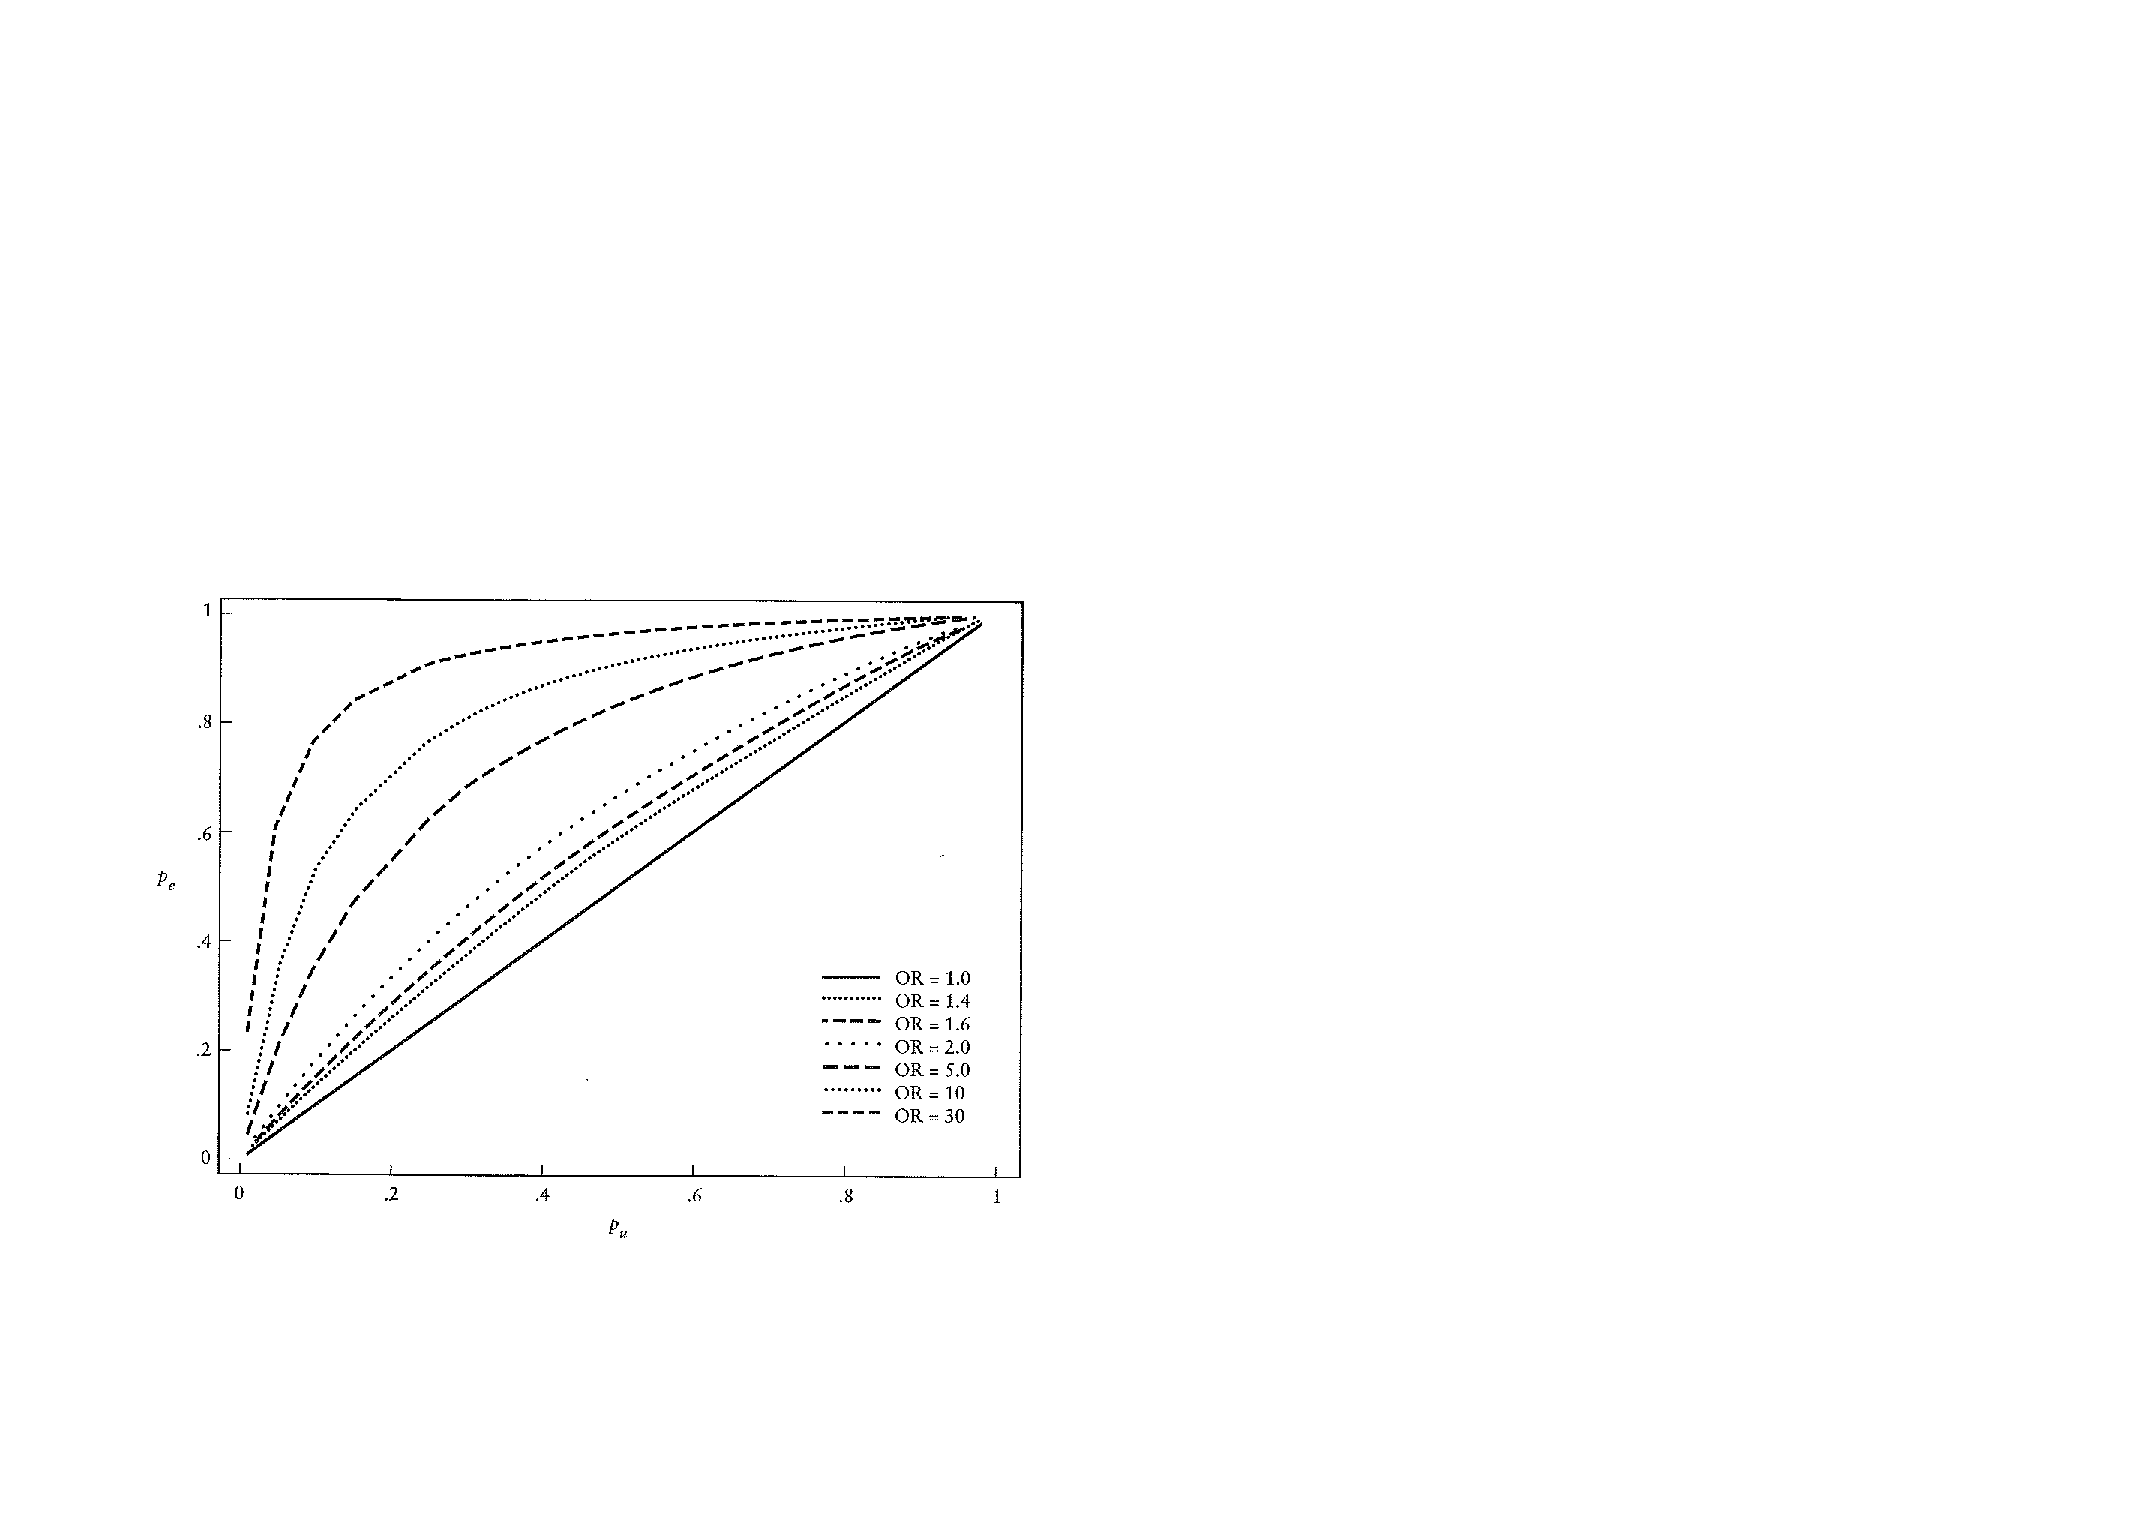
\includegraphics[width=0.85\textwidth]{9-5_logistic_reg/figures/all_OR.pdf}
\end{center}

\end{frame}

%%%%%%%%%%%%%%%%%%%%%%%%%%%%%%%%%%

\subsection{感度と特異度}

%%%%%%%%%%%%%%%%%%%%%%%%%%%%%%%%%%%

\begin{frame}
\frametitle{（昔の）例 --- \emph{House}}

Foxのテレビ番組 \emph{House} を見たことがあれば、House 医師が「ループスであることはない」とよく言うのを知っているだろう。\\
\vspace{3mm}
ループスは、外来細胞を攻撃して感染を防ぐはずの抗体が代わりに血漿タンパク質を外来物として認識し、血栓のリスクが高くなる医学的現象である。人口の 2\% がこの疾患に罹患していると考えられている。\\
\vspace{3mm}
ループスの検査は、実際にループスがある場合は非常に正確だが、ない場合は非常に不正確である。より具体的には、実際に疾患がある人に対して 98\% の精度を持つ。疾患がない人に対しては 74\% の精度を持つ。\\
\vspace{3mm}
ループスの検査が陽性であっても House 医師は正しいか？

\end{frame}

%%%%%%%%%%%%%%%%%%%%%%%%%%%%%%%%%%

\begin{frame}
\frametitle{（昔の）例 --- \emph{House}}

\begin{center}
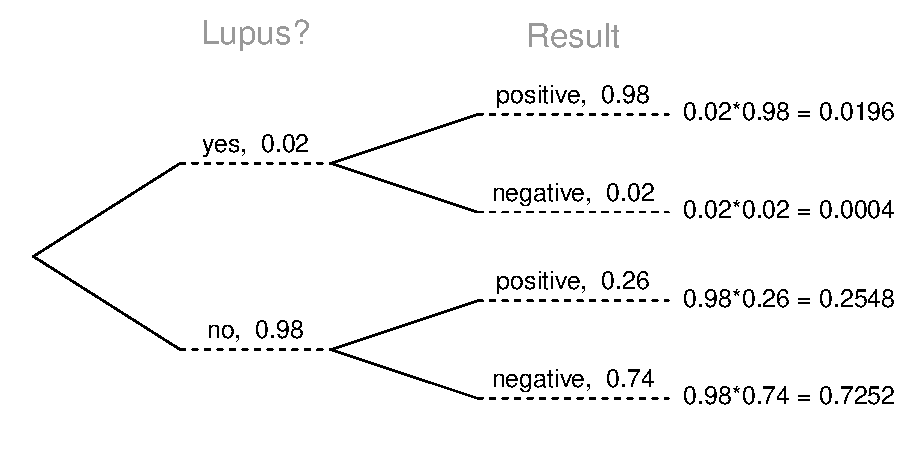
\includegraphics[width=0.8\textwidth]{9-5_logistic_reg/figures/tree_lupus.pdf}
\end{center}

{\footnotesize
\begin{align*}
P(\text{ループス} | +)  &= \frac{P(+,\text{ループス})}{P(+,\text{ループス})+P(+,\text{ループスなし})} \\
                     &= \frac{0.0196}{0.0196+0.2548} = 0.0714
\end{align*}
}
\end{frame}

%%%%%%%%%%%%%%%%%%%%%%%%%%%%%%%%%%

\begin{frame}
\frametitle{ループスの検査}
ループスの検査は実際には非常に複雑で、診断は通常、複数の検査結果に基づく。検査には全血球計算、赤血球沈降速度、腎臓・肝臓評価、尿検査、抗核抗体（ANA）検査などが含まれることが多い。\\
~\\
これらの各検査に何が関わるか（例えば全血球計算が高いか低いかの判断）と、個々の検査および関連する判断が患者へのループス診断の全体的な決定においてどのような役割を果たすかを考えることが重要である。\\

\end{frame}

%%%%%%%%%%%%%%%%%%%%%%%%%%%%%%%%%%

\begin{frame}
\frametitle{ループスの検査}

ある意味で、診断は様々な説明変数の複雑な統合を伴う二値決定（ループスかループスでないか）と見ることができる。\\
~\\
この例は診断がどのように行われるかについての情報を与えてくれないが、与えてくれる同様に重要なことがある --- それが検査の感度と特異度である。これらの値は陽性または陰性の検査結果が実際に何を意味するかを理解するために重要である。

\end{frame}

%%%%%%%%%%%%%%%%%%%%%%%%%%%%%%%%%%

\begin{frame}
\frametitle{感度と特異度}

\hl{感度（Sensitivity）} --- 検査が陽性結果を正しく識別する能力を測定する。
\[P(\text{検査}+~|~\text{疾患}+) = P(+ | \text{ループス}) = 0.98\]

\hl{特異度（Specificity）} --- 検査が陰性結果を正しく識別する能力を測定する。

\[P(\text{検査}-~|~\text{疾患}-) = P(- | \text{ループスなし}) = 0.74\]

\vspace{1cm}

極端なケースについて考えると理解が深まる --- 常に陽性を返す検査の感度と特異度は？常に陰性を返す検査は？

\end{frame}

%%%%%%%%%%%%%%%%%%%%%%%%%%%%%%%%%%

\begin{frame}
\frametitle{感度と特異度（続き）}

\vspace{-5mm}

\begin{center}
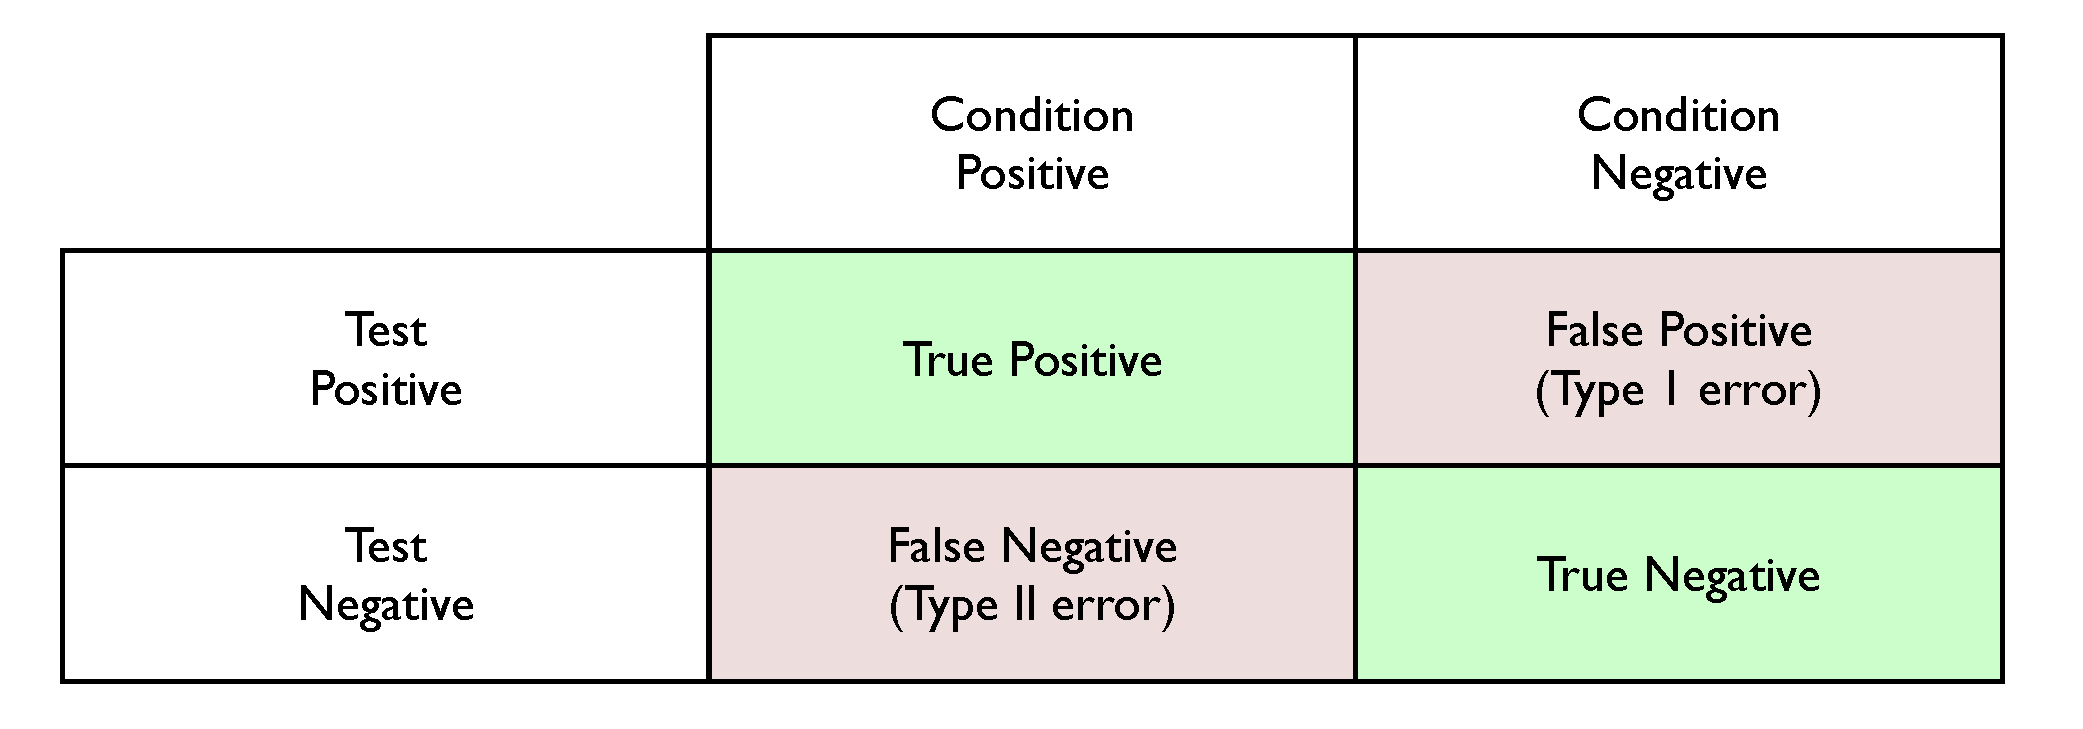
\includegraphics[width=\textwidth]{9-5_logistic_reg/figures/SenSpec.pdf}
\end{center}

\vspace{-9mm}

{\small
\begin{align*}
\text{\hl{感度}} &= P(\text{検査}+~|~\text{疾患}+) = TP / (TP + FN) \\
\text{\hl{特異度}} &= P(\text{検査}-~|~\text{疾患}-) = TN / (FP + TN)\\
\text{\hl{偽陰性率} (\hl{$\beta$})}  &= P(\text{検査}-~|~\text{疾患}+) = FN / (TP + FN) \\
\text{\hl{偽陽性率} (\hl{$\alpha$})} &= P(\text{検査}+~|~\text{疾患}-) = FP / (FP + TN)
\end{align*}

\vspace{-2mm}

\begin{align*}
\text{\hl{感度}} &= 1 - \text{\hl{偽陰性率}} = \text{検出力}\\
\text{\hl{特異度}} &= 1 - \text{\hl{偽陽性率}}
\end{align*}
}

\end{frame}

%%%%%%%%%%%%%%%%%%%%%%%%%%%%%%%%%%

\begin{frame}
\frametitle{それで？}

検査の感度と特異度（および/または偽陽性率と偽陰性率）を知ることが重要であることは明らかである。疾患の有病率（例：$P(\text{ループス})$）とともに、これらの値は $P(\text{ループス}|+)$ のような重要な量を計算するために必要である。\\
~\\
また、第1回中間試験前の検出力分析への簡単な取り組みも、偽陽性率と偽陰性率を最小化することに伴うトレードオフ（検出力を高めるには $\alpha$ または $n$ を増やす必要がある）について示唆を与えているはずである。\\
~\\
意思決定を行おうとするとき、この情報をどのように使うべきか？
\end{frame}

%%%%%%%%%%%%%%%%%%%%%%%%%%%%%%%%%%%

\subsection{ROC 曲線}

%%%%%%%%%%%%%%%%%%%%%%%%%%%%%%%%%%%

\begin{frame}
\frametitle{スパムに戻る}

今週の実験では、スパムメッセージを識別することに関心があるメールのデータセットを調べた。異なる予測変数がメッセージがスパムである確率にどう影響するかを評価するために、異なるロジスティック回帰モデルを検討した。\\

~\\

これらのモデルは受信メッセージに確率を割り当てるためにも使える（これは SLR / MLR の場合の予測に相当する）。しかし、スパムフィルターを設計するとしたら、これは半分の戦いに過ぎない。これらの確率を使って、どのメールをスパムとしてフラグを立てるかについての決定も行う必要がある。\\

~\\

唯一の解決策ではないが、閾値確率を選択し、その確率を超えたメールはスパムとしてフラグを立てるという単純なアプローチを考える。

\end{frame}


%%%%%%%%%%%%%%%%%%%%%%%%%%%%%%%%%%

\begin{frame}
\frametitle{閾値の選択}

\vspace{-5mm}

\begin{center}
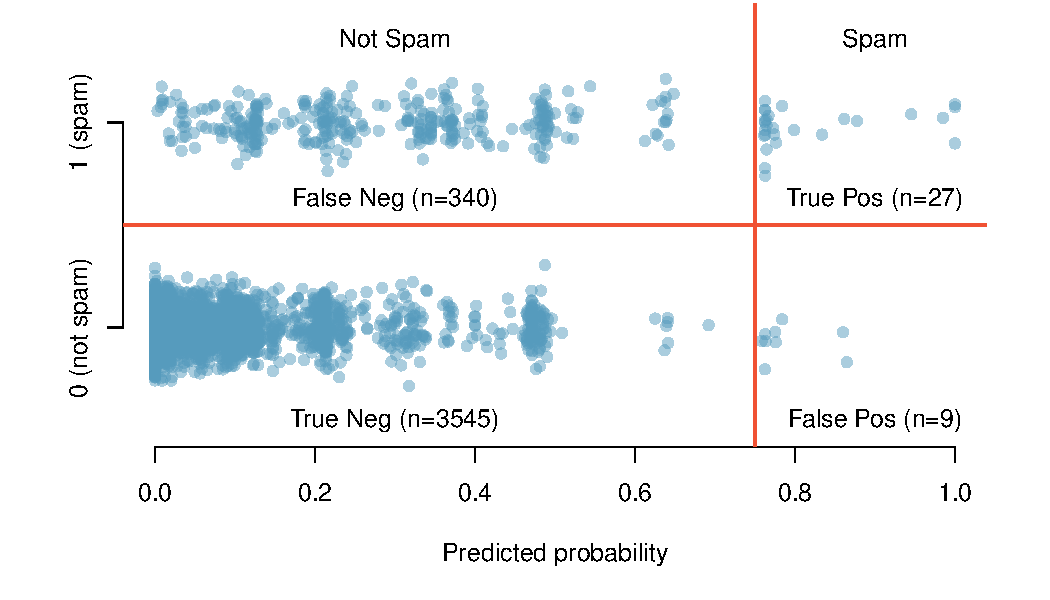
\includegraphics[width=\textwidth]{9-5_logistic_reg/figures/spam/spam5.pdf}
\end{center}

\vspace{-7mm}

\begin{center}
閾値を \orange{0.75} に設定した場合を見てみよう。
\end{center}

\end{frame}

%%%%%%%%%%%%%%%%%%%%%%%%%%%%%%%%%%

\begin{frame}
\frametitle{閾値選択の結果}

メールデータセットで閾値 0.75 を選ぶと以下の結果が得られる：
\vspace{-1.5mm}
\begin{align*}
FN = 340 &\qquad TP = 27 \\
TN = 3545 &\qquad FP = 9
\end{align*}

この意思決定ルールの感度と特異度は？

\soln{
\begin{align*}
\text{感度} & = TP / (TP + FN) = 27 / (27+340) = 0.073 \\
\text{特異度} & = TN / (FP + TN) = 3545 / (9+3545) = 0.997 \\
\end{align*}
}

\end{frame}

%%%%%%%%%%%%%%%%%%%%%%%%%%%%%%%%%%

\begin{frame}
\frametitle{他の閾値を試す}

\vspace{-5mm}

\begin{center}
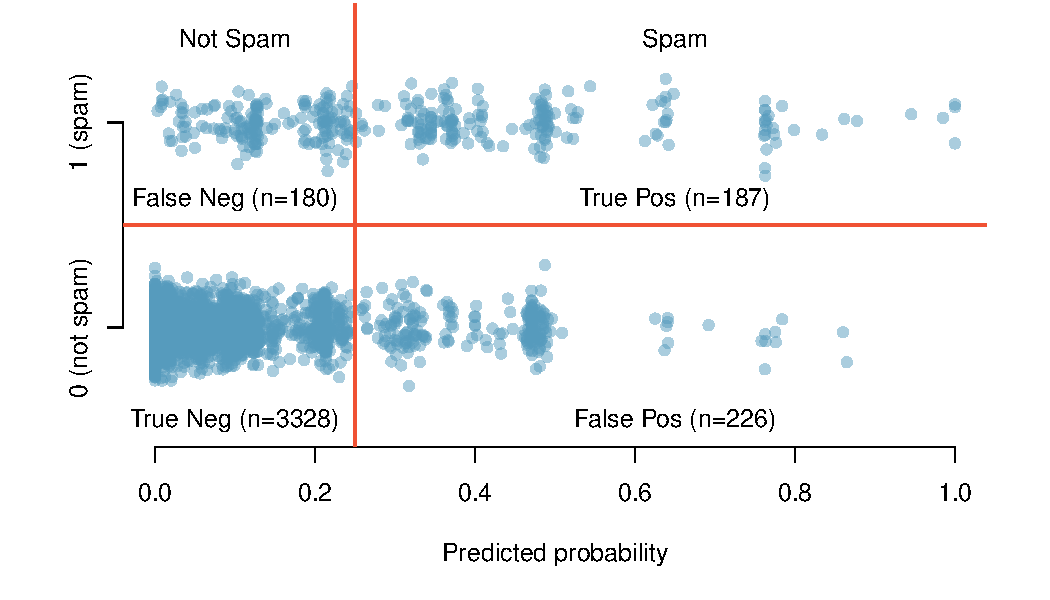
\includegraphics[width=0.9\textwidth]{9-5_logistic_reg/figures/spam/spam5-5.pdf}
\end{center}

{\footnotesize
\begin{center}
\begin{tabular}{|c|ccccc|}
\hline
閾値   & 0.75 & 0.625 & 0.5 & 0.375 & 0.25 \\
\hline
感度 & 0.074 & 0.106 & 0.136 & 0.305 & 0.510 \\
特異度 & 0.997 & 0.995 & 0.995 & 0.963 & 0.936 \\
\hline
\end{tabular}
\end{center}
}

\end{frame}


%%%%%%%%%%%%%%%%%%%%%%%%%%%%%%%%%%

\begin{frame}
\frametitle{感度と特異度の関係}

{\footnotesize
\begin{center}
\begin{tabular}{|c|ccccc|}
\hline
閾値   & 0.75 & 0.625 & 0.5 & 0.375 & 0.25 \\
\hline
感度 & 0.074 & 0.106 & 0.136 & 0.305 & 0.510 \\
特異度 & 0.997 & 0.995 & 0.995 & 0.963 & 0.936 \\
\hline
\end{tabular}
\end{center}
}


\begin{center}
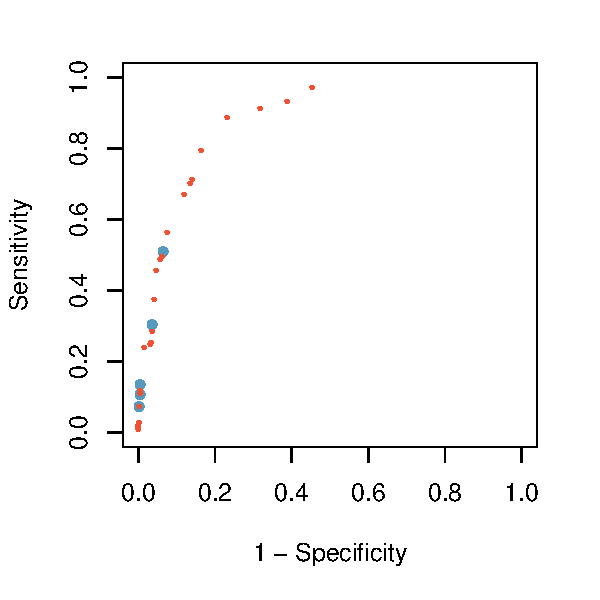
\includegraphics[width=0.5\textwidth]{9-5_logistic_reg/figures/spam/sen_vs_spec3.pdf}
\end{center}

\end{frame}

%%%%%%%%%%%%%%%%%%%%%%%%%%%%%%%%%%

\begin{frame}
\frametitle{受信者操作特性（ROC）曲線}

\vspace{-8mm}

\begin{center}
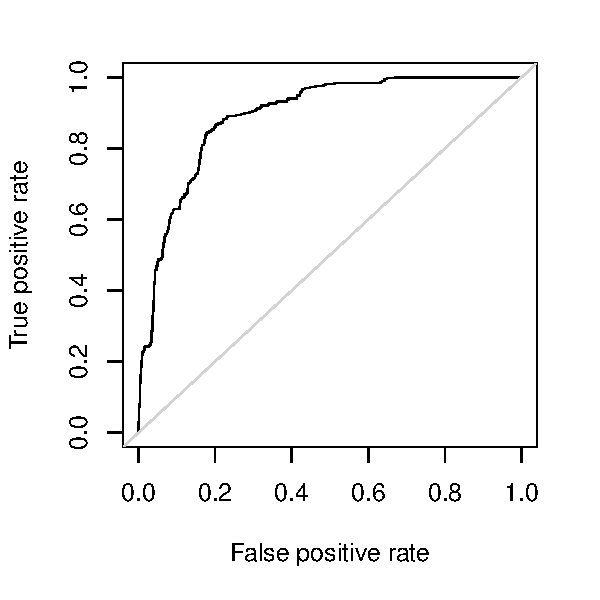
\includegraphics[width=0.7\textwidth]{9-5_logistic_reg/figures/spam/ROC.pdf}
\end{center}

\end{frame}

%%%%%%%%%%%%%%%%%%%%%%%%%%%%%%%%%%

\begin{frame}
\frametitle{受信者操作特性（ROC）曲線（続き）}

なぜ ROC 曲線を使うのか？

\begin{itemize}
\item すべての可能な閾値における感度と特異度のトレードオフを示す。

\item 偶然による性能との比較が直感的にわかる。

\item 曲線下面積（AUC）をモデルの予測能力の評価として使用できる。

\end{itemize}

\end{frame}

%%%%%%%%%%%%%%%%%%%%%%%%%%%%%%%%%%

\begin{frame}[fragile]
\frametitle{スパムモデルの精緻化}

\vspace{-5mm}

{\footnotesize
\begin{verbatim}
g_refined = glm(spam ~ to_multiple+cc+image+attach+winner
                      +password+line_breaks+format+re_subj
                      +urgent_subj+exclaim_mess,
                data=email, family=binomial)
summary(g_refined)
\end{verbatim}

\begin{center}
\begin{tabular}{rrrrr}
  \hline
 & Estimate & Std. Error & z value & Pr($>$$|$z$|$) \\
  \hline
(Intercept) & -1.7594 & 0.1177 & -14.94 & 0.0000 \\
  to\_multipleyes & -2.7368 & 0.3156 & -8.67 & 0.0000 \\
  ccyes & -0.5358 & 0.3143 & -1.71 & 0.0882 \\
  imageyes & -1.8585 & 0.7701 & -2.41 & 0.0158 \\
  attachyes & 1.2002 & 0.2391 & 5.02 & 0.0000 \\
  winneryes & 2.0433 & 0.3528 & 5.79 & 0.0000 \\
  passwordyes & -1.5618 & 0.5354 & -2.92 & 0.0035 \\
  line\_breaks & -0.0031 & 0.0005 & -6.33 & 0.0000 \\
  formatPlain & 1.0130 & 0.1380 & 7.34 & 0.0000 \\
  re\_subjyes & -2.9935 & 0.3778 & -7.92 & 0.0000 \\
  urgent\_subjyes & 3.8830 & 1.0054 & 3.86 & 0.0001 \\
  exclaim\_mess & 0.0093 & 0.0016 & 5.71 & 0.0000 \\
   \hline
\end{tabular}
\end{center}

}
\end{frame}

%%%%%%%%%%%%%%%%%%%%%%%%%%%%%%%%%%

\begin{frame}[fragile]
\frametitle{モデルの比較}

\vspace{-8mm}

\begin{center}
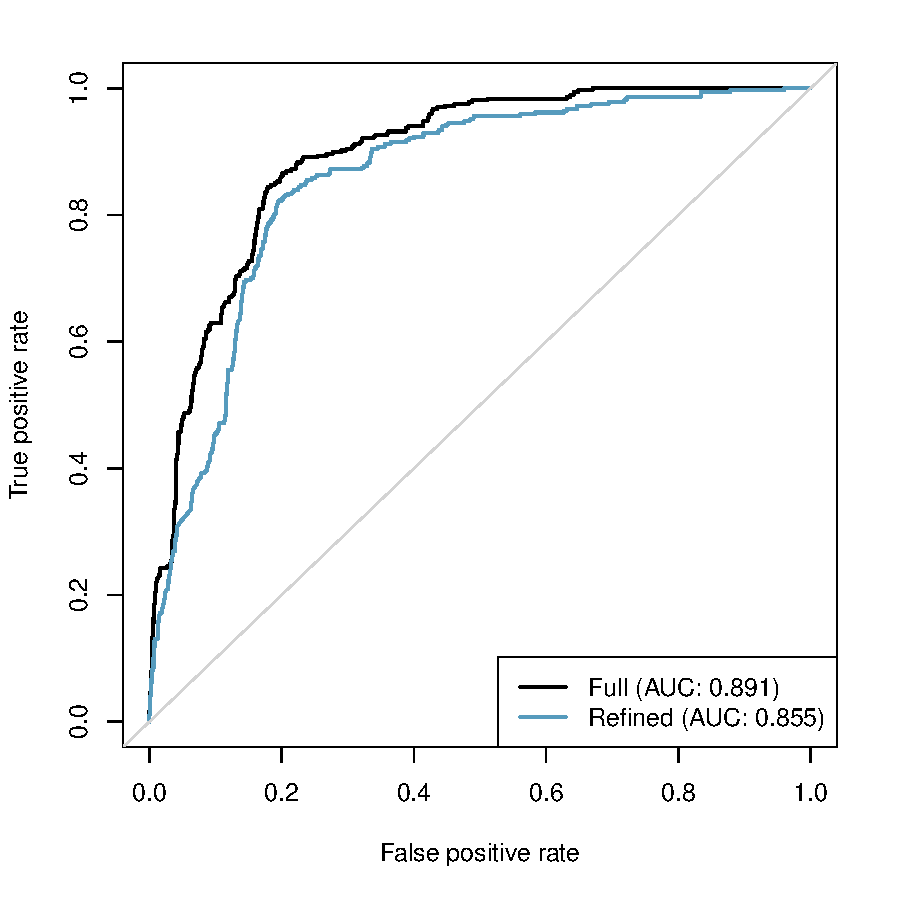
\includegraphics[width=0.7\textwidth]{9-5_logistic_reg/figures/spam/ROC_comp.pdf}
\end{center}

\end{frame}

%%%%%%%%%%%%%%%%%%%%%%%%%%%%%%%%%%

\subsection{効用関数}

%%%%%%%%%%%%%%%%%%%%%%%%%%%%%%%%%%%

\begin{frame}
\frametitle{効用関数}

「最良の」閾値を決定するために使える合理的な定量的アプローチは他にも多くある。\\
~\\
経済学のコースを受けたことがあれば、効用関数のアイデアを聞いたことがあるだろう。各結果に対してコストと利益を割り当て、各状況の効用を計算するためにそれらを使うことができる。

\end{frame}

%%%%%%%%%%%%%%%%%%%%%%%%%%%%%%%%%%

\begin{frame}
\frametitle{スパムフィルターの効用関数}

スパムフィルターの効用関数を記述するには、各結果のコスト/利益を考慮する必要がある。

\begin{center}
 \renewcommand\arraystretch{1.5}
\begin{tabular}{l|c}
結果 & 効用 \\
\hline
真陽性（TP）  & 1 \\
真陰性（TN）  & 1 \\
偽陽性（FP） & -50 \\
偽陰性（FN） & -5 \\
\end{tabular}
\end{center}
~\\
\[U(p) = TP(p) + TN(p) - 50 \times FP(p) - 5 \times FN(p)\]

\end{frame}

%%%%%%%%%%%%%%%%%%%%%%%%%%%%%%%%%%

\begin{frame}
\frametitle{閾値 0.75 の効用}

メールデータセットで閾値 0.75 を選ぶと以下の結果が得られる：
\vspace{-1.5mm}
\begin{align*}
FN = 340 &\qquad TP = 27 \\
TN = 3545 &\qquad FP = 9
\end{align*}

\begin{align*}
U(p) &= TP(p) + TN(p) - 50 \times FP(p) - 5 \times FN(p) \\
     &= 27+3545-50\times9-5\times340 = 1422
\end{align*}

それ自体では有用ではないが、他の閾値と比較することができる。

\end{frame}

%%%%%%%%%%%%%%%%%%%%%%%%%%%%%%%%%%

\begin{frame}
\frametitle{効用曲線}

\vspace{-5mm}

\begin{center}
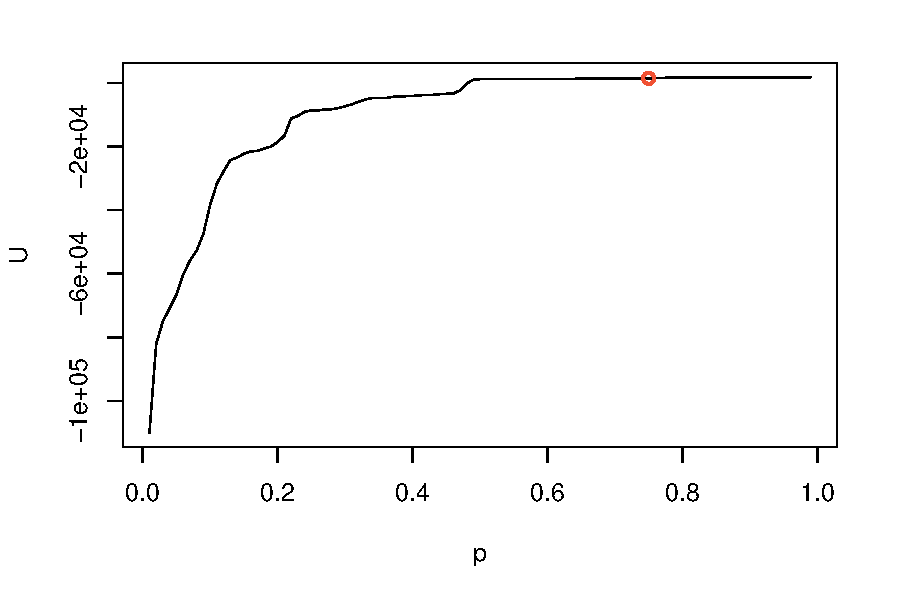
\includegraphics[width=\textwidth]{9-5_logistic_reg/figures/spam/utility.pdf}
\end{center}

\end{frame}


%%%%%%%%%%%%%%%%%%%%%%%%%%%%%%%%%%

\begin{frame}
\frametitle{効用曲線（拡大）}

\vspace{-5mm}

\begin{center}
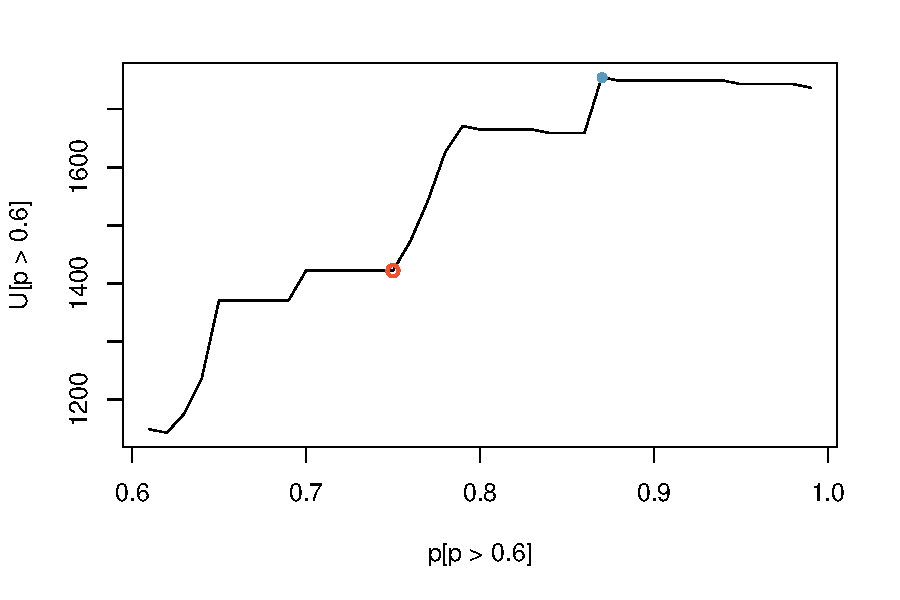
\includegraphics[width=\textwidth]{9-5_logistic_reg/figures/spam/utility3.pdf}
\end{center}

\end{frame}

%%%%%%%%%%%%%%%%%%%%%%%%%%%%%%%%%%

\begin{frame}
\frametitle{最大効用}

\begin{center}
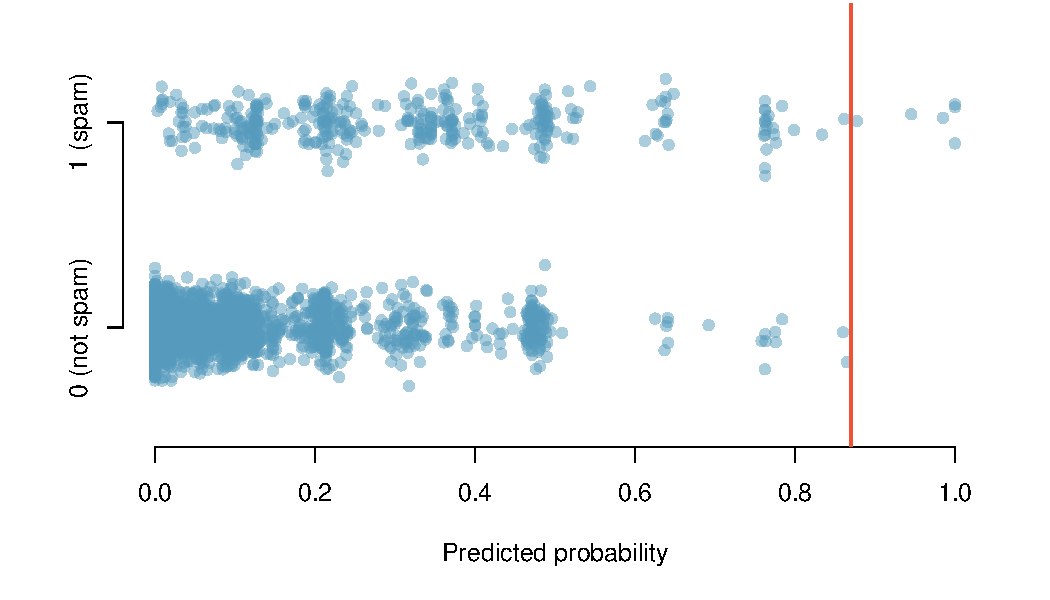
\includegraphics[width=\textwidth]{9-5_logistic_reg/figures/spam/utility4.pdf}
\end{center}

\end{frame}
